\documentclass[letter,11pt]{article}

\usepackage[spanish,es-nodecimaldot]{babel}
\usepackage[utf8]{inputenc}

\usepackage{lmodern}
\usepackage[T1]{fontenc}
\usepackage{textcomp}

\usepackage{framed}
\usepackage[svgnames]{xcolor}
\colorlet{shadecolor}{Gainsboro!50}

\usepackage[labelfont=bf]{caption}
\usepackage{graphicx}
\usepackage{pstricks}

\usepackage{anysize}
\marginsize{3cm}{2cm}{2cm}{3cm}

\usepackage{siunitx}
\usepackage{amsmath}
\usepackage{array}
\usepackage{csquotes}

\usepackage{fancyhdr}
\usepackage{lastpage}
\pagestyle{fancy}
\fancyhf{}
\fancyhead[LE,RO]{Laboratorio de Circuitos Eléctricos I}
\fancyfoot[CO,CE]{\thepage\ de \pageref{LastPage}}

\special{papersize=215.9mm,279.4mm}

\usepackage[
    pdfauthor={Carlos Eduardo Caballero Burgoa},%
    pdftitle={Laboratorio de Circuitos Eléctricos I},%
    pdfsubject={Teorema de Superposición},%
    colorlinks,%
    citecolor=black,%
    filecolor=black,%
    linkcolor=black,%
    urlcolor=black,
    breaklinks]{hyperref}
\usepackage{breakurl}

\newcommand{\blankpage}{
\newpage
\thispagestyle{empty}
\mbox{}
\newpage
}

\renewcommand{\arraystretch}{1.2}

\begin{document}

\begin{titlepage}
    \begin{center}
        {\Large UNIVERSIDAD MAYOR DE SAN SIMÓN}\\
        \vspace*{0.15cm}
        {\large FACULTAD DE CIENCIAS Y TECNOLOGÍA}\\
        \vspace*{0.10cm}
        DEPARTAMENTO DE ELÉCTRICA-ELECTRÓNICA\\
        \vspace*{3.0cm}
        {\Large \textbf{LABORATORIO DE CIRCUITOS ELÉCTRICOS I}}\\
        \vspace*{0.3cm}
        {\Large \textbf{INFORME No. 6}}\\
        \vspace*{3.5cm}
        {\Large \textbf{TEOREMA DE SUPERPOSICIÓN}}\\
    \end{center}

    \vspace*{6.4cm}
    \leftskip=7.95cm
    \noindent
    \textbf{Estudiante:}\\
    Caballero Burgoa, Carlos Eduardo.\\
    \newline
    \textbf{Carrera:}\\
    Ing. Electromecánica.\\
    \newline
    \textbf{Docente:}\\
    Ing. Marco Antonio Vallejo Camacho.\\
    \newline
    \textbf{Grupo:} 3E.\\
    \textbf{Fecha de entrega:} 11 de Junio del 2024.\\
\end{titlepage}

\section{Cálculos previos}

\vspace{1.0cm}
\begin{figure}[!h]
\centering
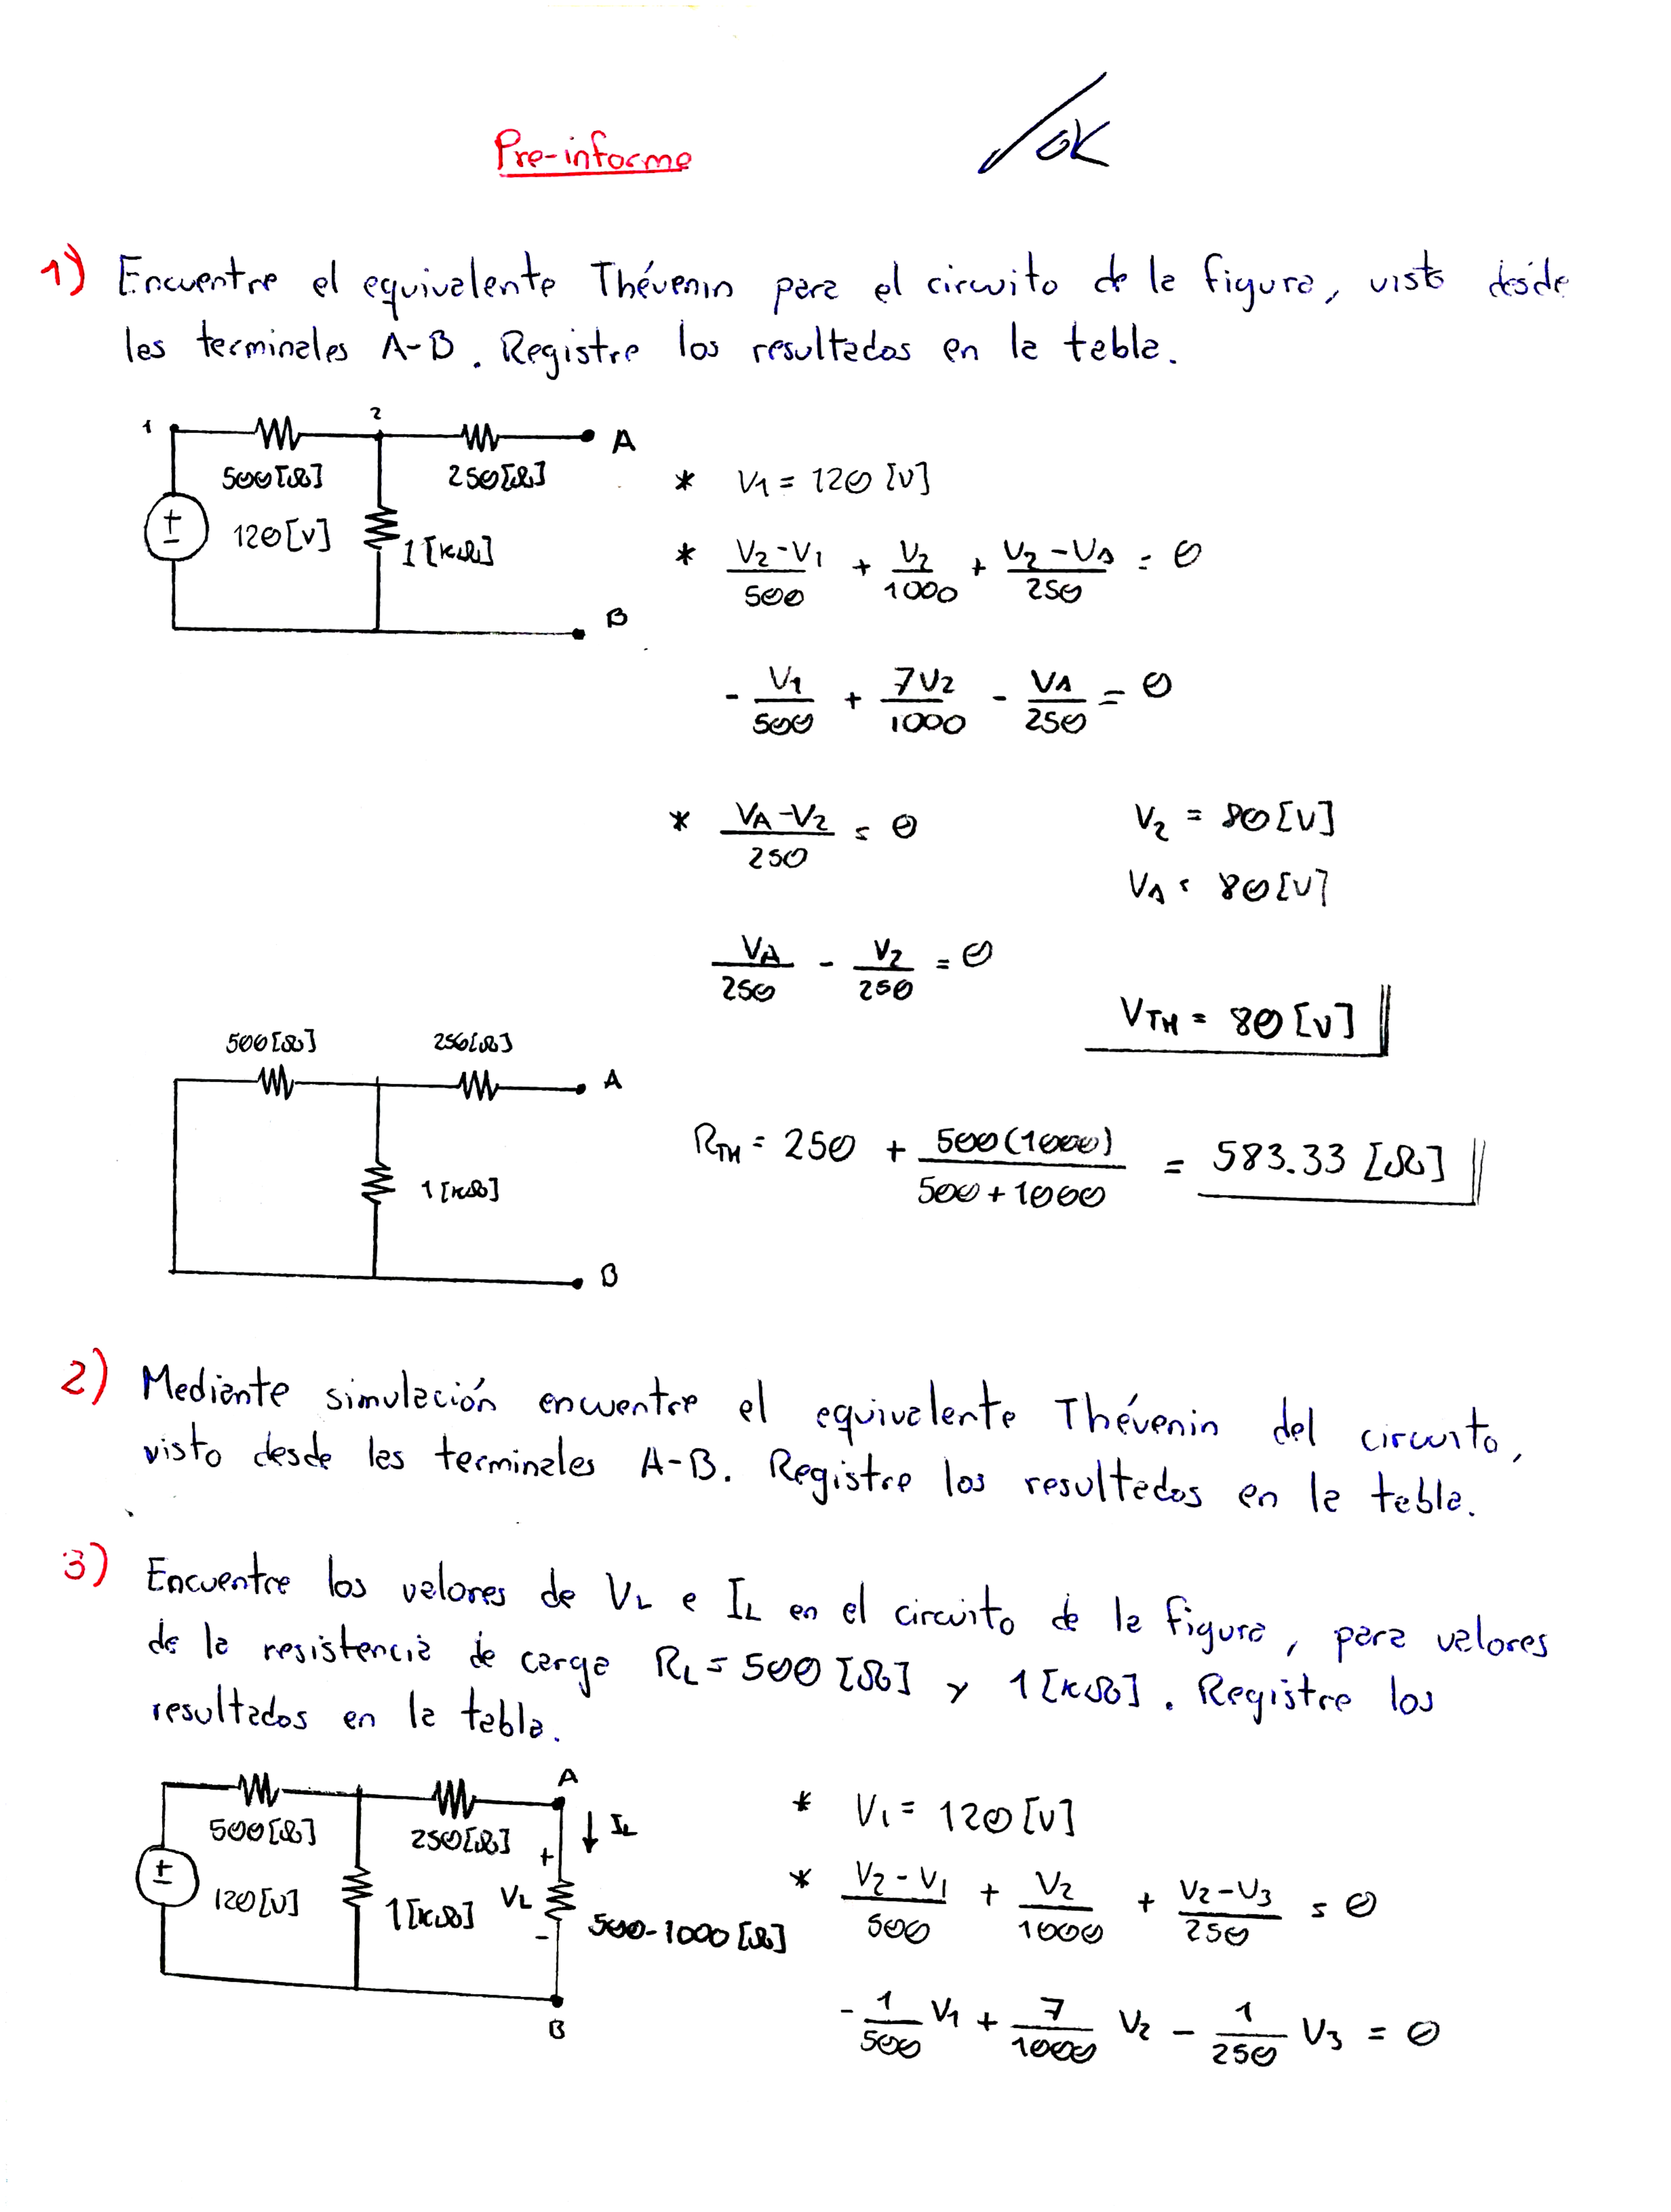
\includegraphics[scale=0.18]{resources/preinforme1.eps}
\end{figure}

\newpage

\begin{figure}[!h]
\centering
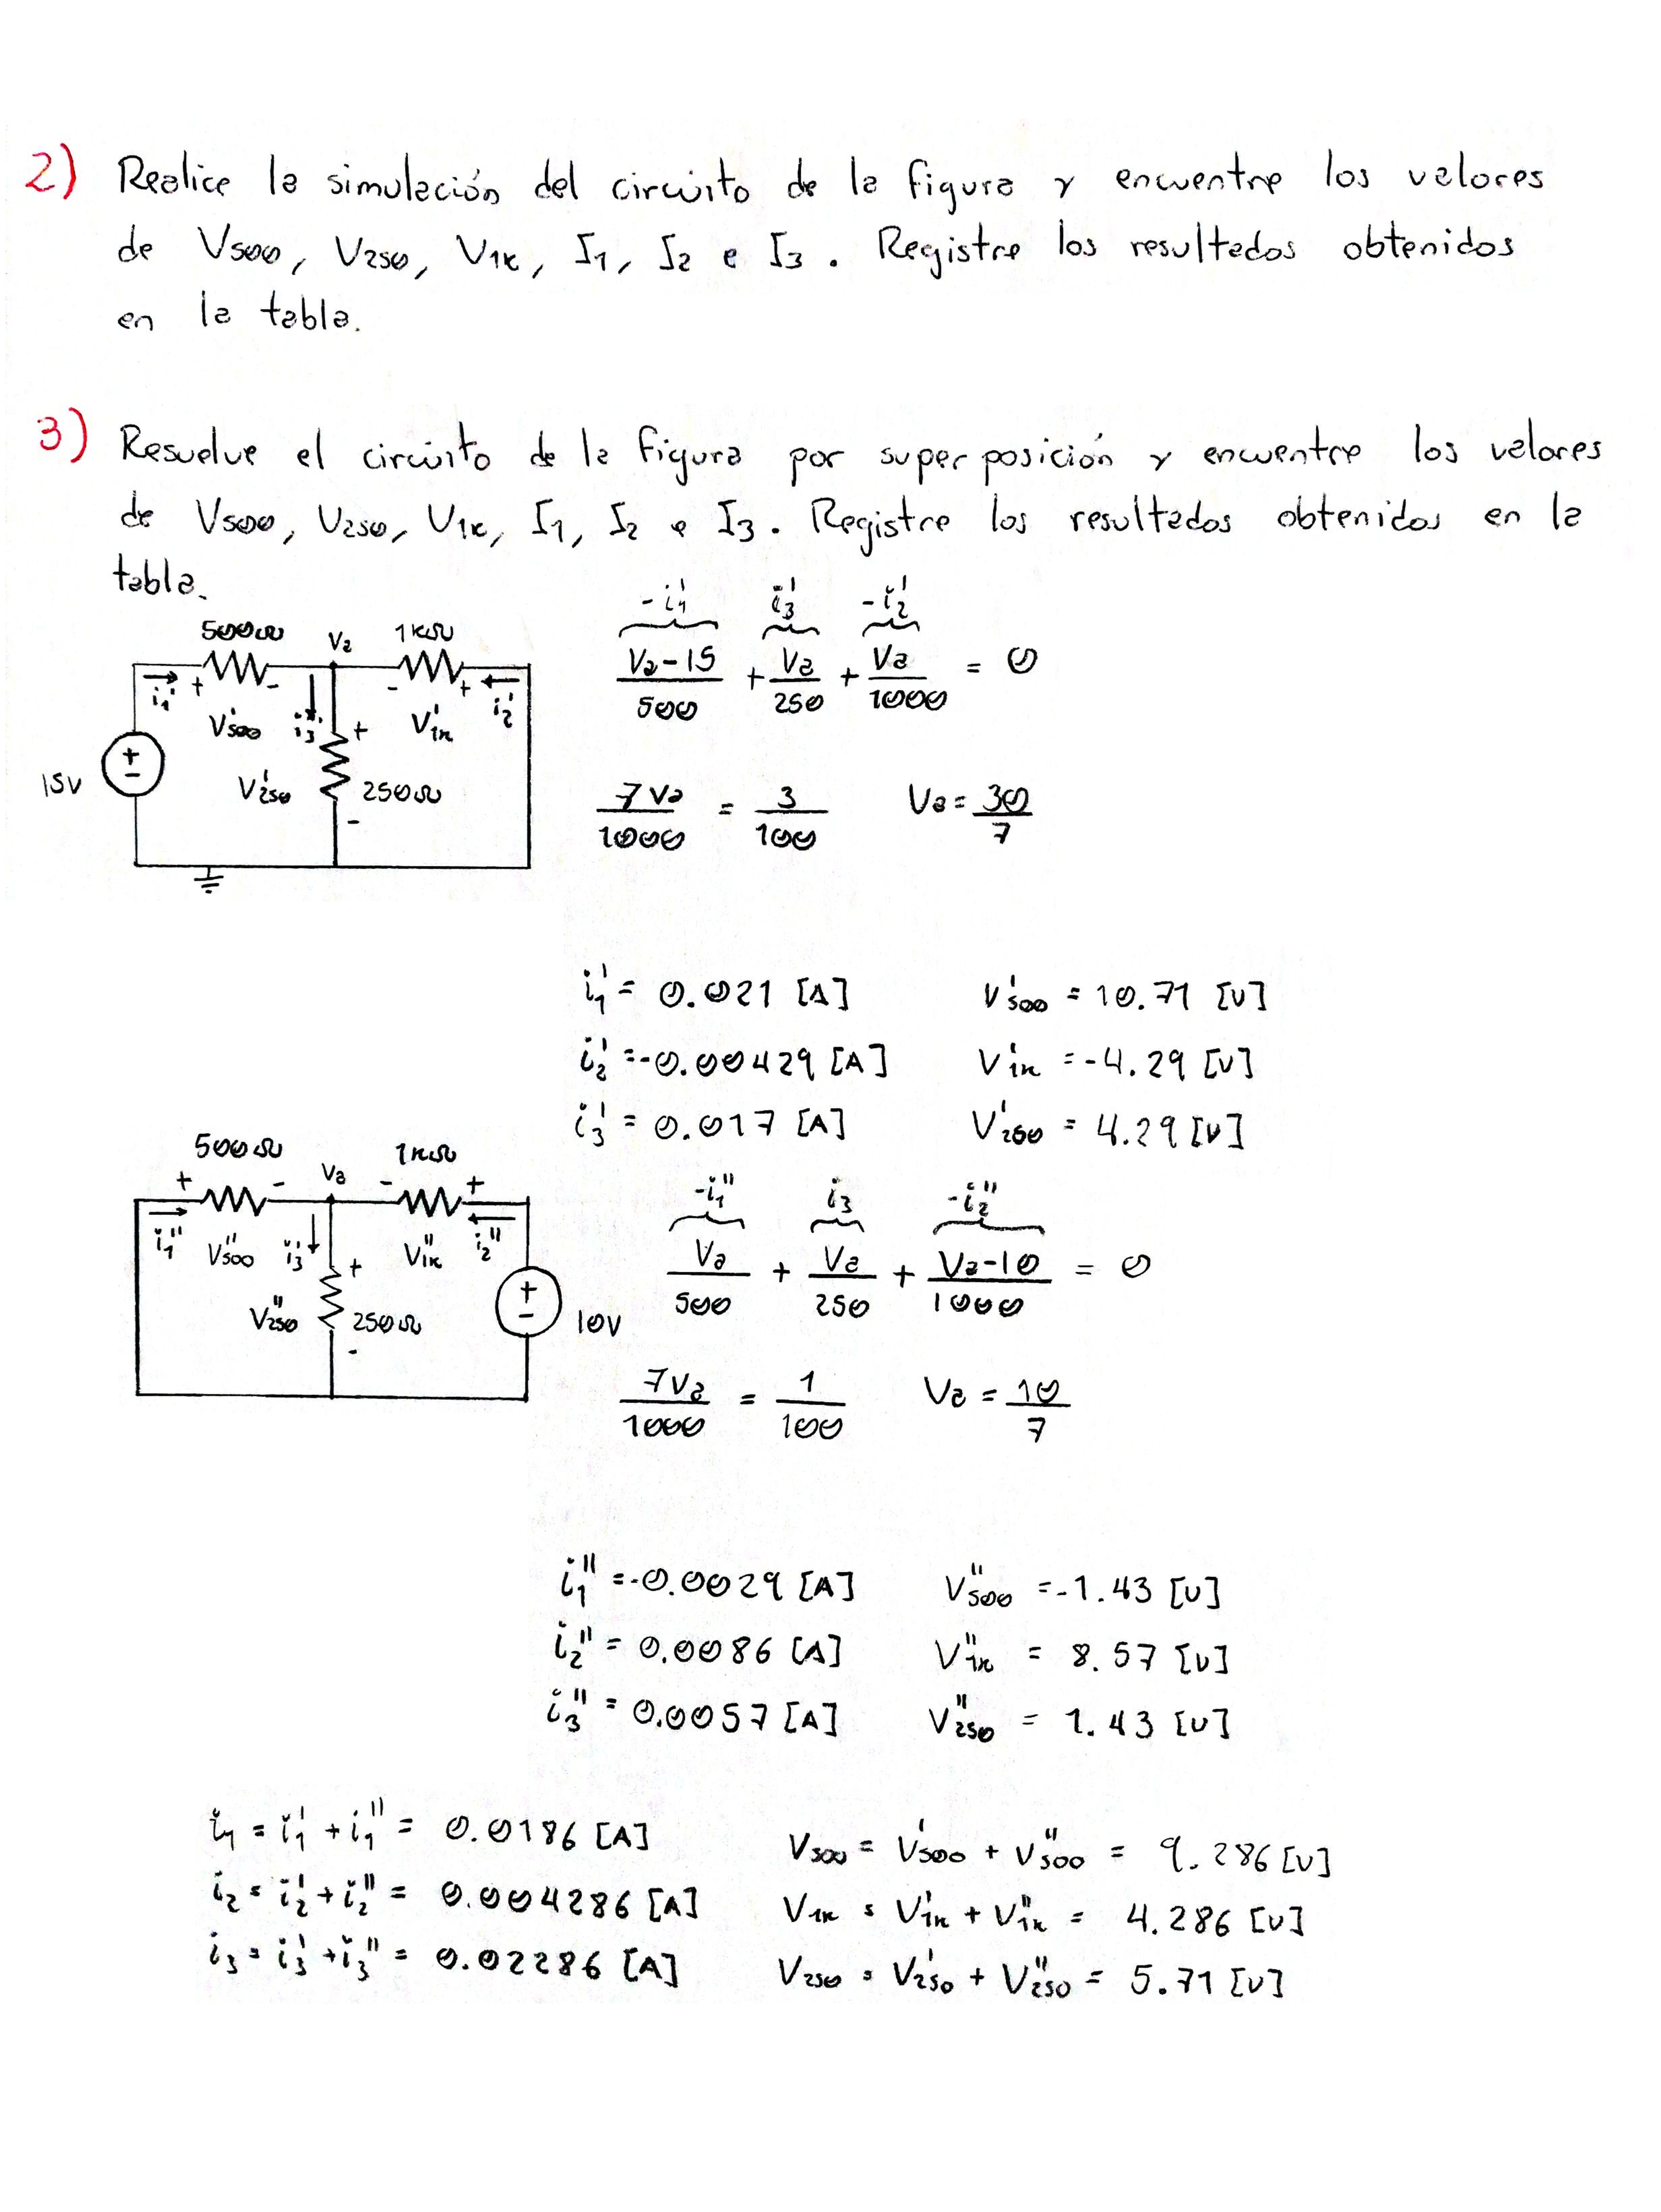
\includegraphics[scale=0.18]{resources/preinforme2.eps}
\end{figure}

\section{Simulación}
Se utilizó el software \emph{Quite Universal Circuit Simulator.} para simular
los circuitos, estos pueden verse en la figura (\ref{simulacion1}),
(\ref{simulacion2}) y (\ref{simulacion3}).
\\

\begin{figure}[!h]
\centering
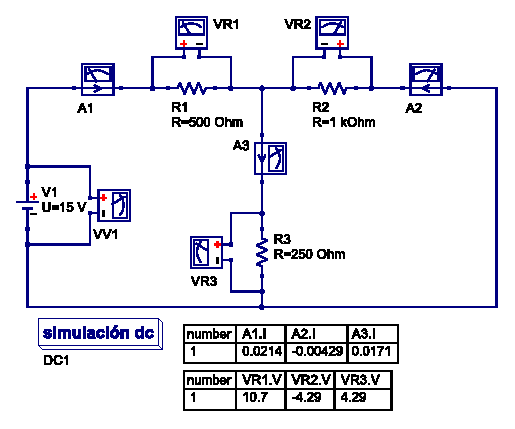
\includegraphics[scale=1.27]{simulation/practica6.1.eps}
\caption{Simulación del circuito con la fuente de $15[V]$.}
\label{simulacion1}
\end{figure}

\begin{figure}[!h]
\centering
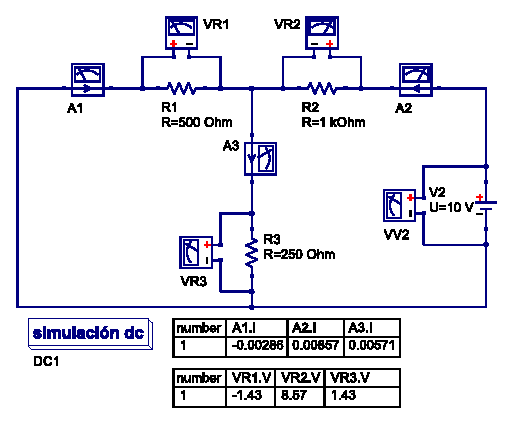
\includegraphics[scale=1.27]{simulation/practica6.2.eps}
\caption{Simulación del circuito con la fuente de $10[V]$.}
\label{simulacion2}
\end{figure}

\newpage

\begin{figure}[!h]
\centering
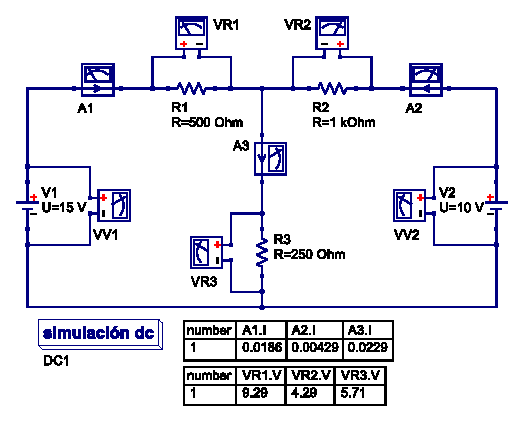
\includegraphics[scale=1.27]{simulation/practica6.eps}
\caption{Simulación del circuito con las dos fuentes de tensión.}
\label{simulacion3}
\end{figure}

\newpage

\section{Tablas y mediciones}
En la figura (\ref{tablas}), se adjunta la hoja de resultados provista en la
guía de laboratorio, rellenada con la información teórica, simulada y las
mediciones realizadas en laboratorio.

\begin{figure}[!h]
\centering
\includegraphics[scale=0.20]{resources/preinforme3.eps}
\caption{Tabla de resultados.}
\label{tablas}
\end{figure}

\section{Cuestionario}

\begin{enumerate}

\item \textbf{En el circuito presentado en la figura a continuación, determine
el valor del parámetro adimensional $\alpha$, aplicando el teorema de
superposición, tal que el voltaje $V_x = 0 [V]$.}

\begin{figure}[!h]
\centering
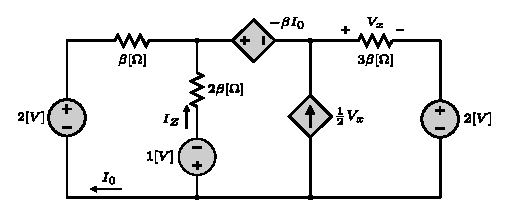
\includegraphics[width=0.6\textwidth]{resources/figura1.eps}
\end{figure}

Se calcula $V_x$ para la fuente de corriente de $6[A]$:

\begin{figure}[!h]
\centering
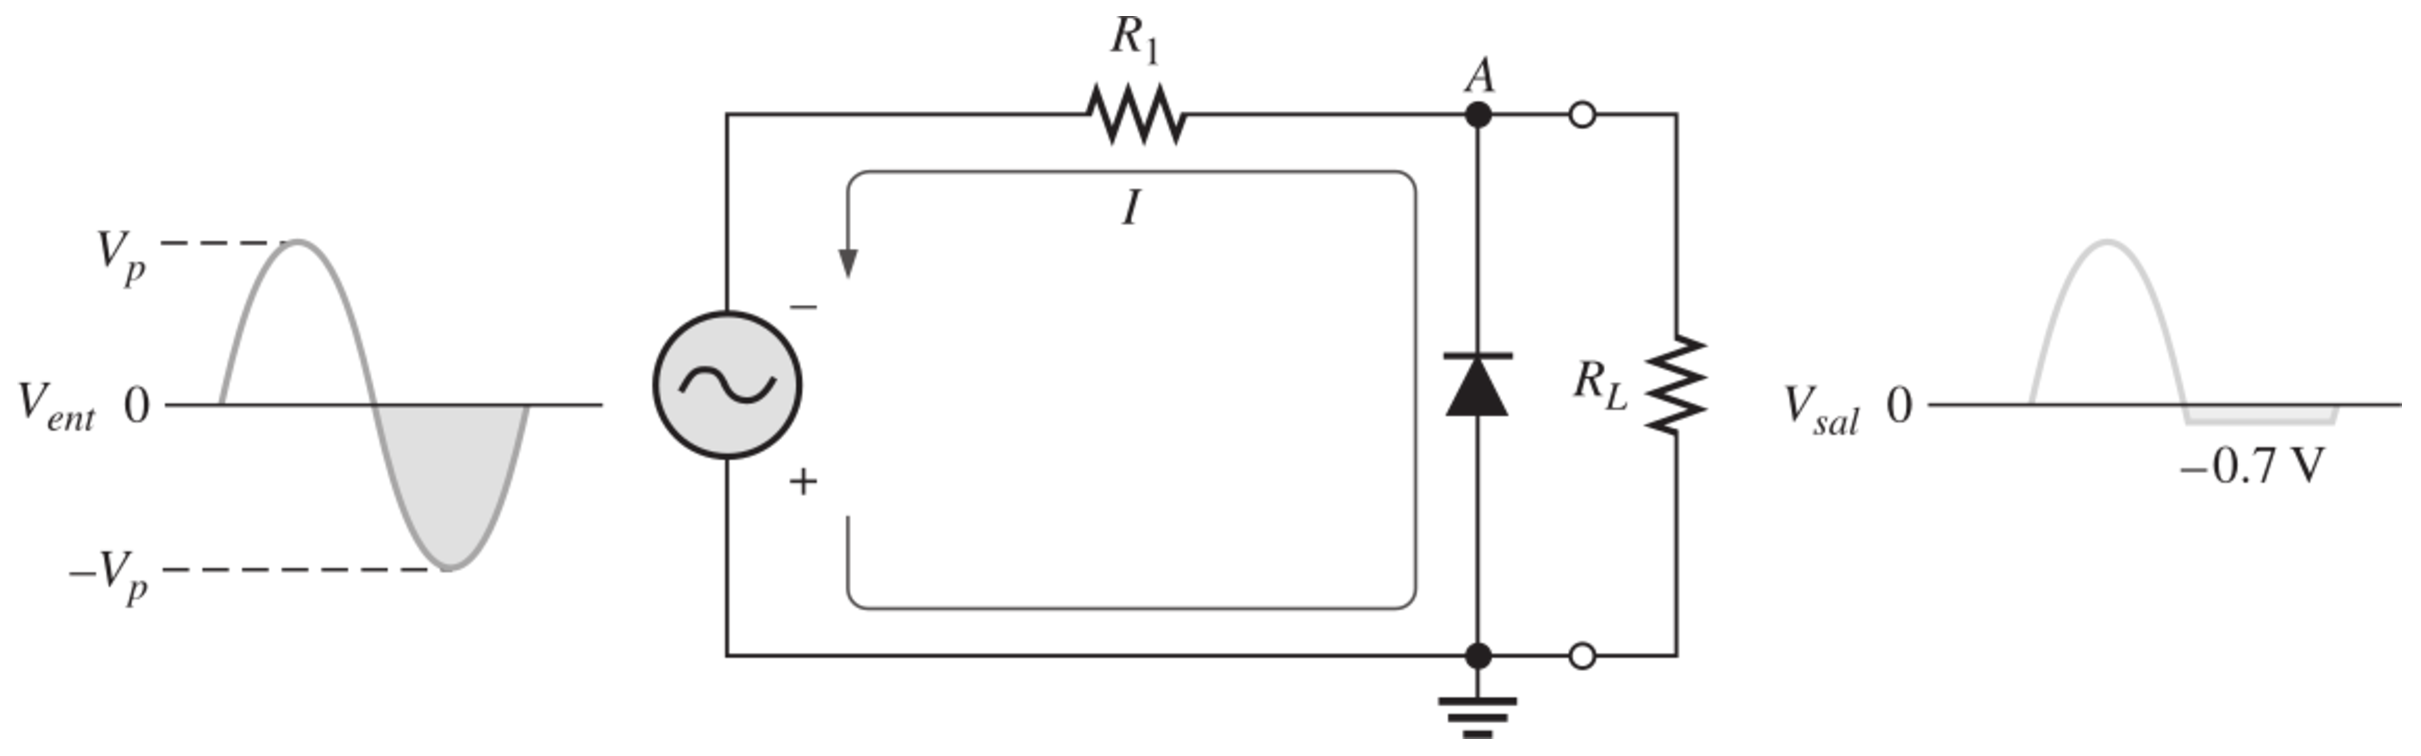
\includegraphics[width=0.35\textwidth]{resources/figura2.eps}
\end{figure}

Usando el método de tensiones de malla con la supermalla, se obtiene:

\begin{equation}
    3\alpha i_1 + \alpha i_2 - V_0 + 2\alpha i_2 = 0
    \label{ec1.1}
\end{equation}

Se sabe que $i_2 = 6$, por tanto:

\begin{equation*}
    i_2 - i_1 = V_0
\end{equation*}
\begin{equation}
    i_1 = 6 - V_0
    \label{ec1.2}
\end{equation}

Reemplazando (\ref{ec1.2}) en (\ref{ec1.1}):

\begin{equation*}
    3\alpha (6 - V_0) + 6 \alpha - V_0 + 12\alpha = 0
\end{equation*}
\begin{equation*}
    18\alpha - 3\alpha V_0 + 6 \alpha - V_0 + 12\alpha = 0
\end{equation*}
\begin{equation*}
    36\alpha - 3\alpha V_0 - V_0 = 0
\end{equation*}
\begin{equation*}
    V_0 (3\alpha + 1) = 36\alpha
\end{equation*}
\begin{equation}
    V_0 = \frac{36\alpha}{3\alpha + 1}
    \label{ec1.3}
\end{equation}

Se calcula $V_x$ en función de $\alpha$:

\begin{equation*}
    V_x = 3\alpha i_1
\end{equation*}
\begin{equation}
    V_x = 3\alpha (6 - V_0)
    \label{ec1.4}
\end{equation}

Reemplazando (\ref{ec1.3}) en (\ref{ec1.4}):

\begin{equation}
    V_x = 3\alpha \left(6 - \frac{36\alpha}{3\alpha + 1}\right)
    \label{ec1.5}
\end{equation}

Se calcula $V_x$ para la fuente de tensión de $12[V]$:

\begin{figure}[!h]
\centering
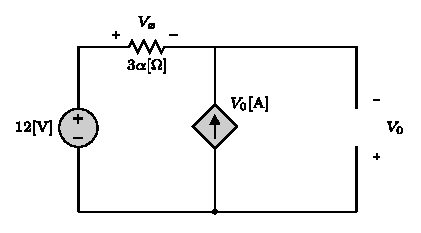
\includegraphics[width=0.41\textwidth]{resources/figura3.eps}
\end{figure}

Usando el método de tensiones de malla, se obtiene:

\begin{equation}
    -12 + 3\alpha i_1 + V_{V_0} = 0
    \label{ec2.1}
\end{equation}

Se sabe que $i_1 = V_0$ y que $V_{V_0} = V_0$, por tanto:

\begin{equation*}
    -12 + 3\alpha V_0 + V_0 = 0
\end{equation*}
\begin{equation*}
    3\alpha V_0 + V_0 = 12
\end{equation*}
\begin{equation*}
    V_0 (3\alpha + 1) = 12
\end{equation*}
\begin{equation}
    V_0 = \frac{12}{3\alpha + 1}
    \label{ec2.2}
\end{equation}

Se calcula $V_x$ en función de $\alpha$:

\begin{equation*}
    V_x = 3\alpha i_1
\end{equation*}
\begin{equation}
    V_x = 3\alpha V_0
    \label{ec2.3}
\end{equation}

Reemplazando (\ref{ec2.2}) en (\ref{ec2.3}):

\begin{equation}
    V_x = \frac{36\alpha}{3\alpha + 1}
    \label{ec2.4}
\end{equation}

Para que $V_x = 0$:

\begin{equation*}
    3\alpha \left(6 - \frac{36\alpha}{3\alpha + 1}\right) + \frac{36\alpha}{3\alpha + 1} = 0
\end{equation*}
\begin{equation*}
    18\alpha - \frac{108\alpha}{3\alpha + 1} + \frac{36\alpha}{3\alpha + 1} = 0
\end{equation*}
\begin{equation*}
    18\alpha = \frac{72\alpha}{3\alpha + 1}
\end{equation*}
\begin{equation*}
    3\alpha + 1 = 4
\end{equation*}
\begin{equation}
    \alpha = 1
\end{equation}

\end{enumerate}

\section{Conclusiones}
Se demostró experimentalmente el principio de superposición, mediante la
medición de circuitos tanto en laboratorio, como mediante una simulación.

Es de destacar en las mediciones de laboratorio, que la suma algebraica de las
tensiones y las corrientes, son muy precisas respecto a la medición con las dos
fuentes de tensión, esto puede deberse al correcto manejo de las escalas en el
multímetro, y las cantidades pequeñas involucradas en el experimento.

\begin{center}
\begin{tabular}{|c||c||c|c|c||c|}
\hline
& \textbf{Dos fuentes} &
    \textbf{Fuente $15[\text{V}]$} &
    \textbf{Fuente $10[\text{V}]$} &
    \textbf{Suma algebraica} &
    \textbf{Error}
\tabularnewline \hline \hline
$V_{500[\Omega]}$ & 9.60[V] & 10.97[V] & -1.37[V] & 9.6[V] & $0\%$
\tabularnewline \hline
$V_{250[\Omega]}$ & 5.60[V] & 4.22[V] & 1.38[V] & 5.6[V] & $0\%$
\tabularnewline \hline
$V_{1[k\Omega]}$ & 4.35[V] & -4.22[V] & 8.56[V] & 4.34[V] & $0.23\%$
\tabularnewline \hline
\end{tabular}
\end{center}

\begin{center}
\begin{tabular}{|c||c||c|c|c||c|}
\hline
& \textbf{Dos fuentes} &
    \textbf{Fuente $15[\text{V}]$} &
    \textbf{Fuente $10[\text{V}]$} &
    \textbf{Suma algebraica} &
    \textbf{Error}
\tabularnewline \hline \hline
$I_1$ & 18.6[mA] & 20.9[mA] & -2.6[mA] & 18.3[mA] & $0.016\%$
\tabularnewline \hline
$I_2$ & 22.7[mA] & 16.9[mA] & 5.5[mA] & 22.4[mA] & $0.013\%$
\tabularnewline \hline
$I_3$ & 4.1[mA] & -4[mA] & 8.2[mA] & 4.2[mA] & $0.024\%$
\tabularnewline \hline
\end{tabular}
\end{center}

\end{document}

